\section{Java}
Java je jedním z nejpoužívanějších a nejpopulárnějších počítačových programovacích jazyků na světě. Syntaxe tohoto jazyka se řadí k těm jednodužším, avšak jeho použití je velmi rozsáhlé. V Java se programují čipové karty, mobilní a desktopové aplikace, i velké podnikové a informační systémy. Java je jazyk multiplatformní a díky tomu je jej možné použít ná různých operačních systémech. Java je vyvíjena jako OpenSource. Java se objevuje ve třech základních edicích:


\subsection{Java platformy}
Jazyk Java je společně s virtuálním strojem a knihovnami vydáván ve čtyřech platformách, kde každá má své speciální určení.

\subsubsection{Java SE}
Základní platforma pro vývoj desktopových a jednodužších serverových aplikací. V součané době je poslední vydaná verze Java SE 8u25.

\subsubsection{Java EE}
Nádstavba nad Java SE obsahující speciální knihovny pro vývoj a provoz podnikových aplikací a informačních systémů. V součané době je poslední vydaná verze Java EE 7.

\subsubsection{Java ME (Micro Edition)}
Podmnožina Java SE pro vývoj aplikací pro malá zařízení jako jsou mikrokontroléry sensory, mobilní telefony, set-top boxy, tiskárny a další. V součané době je poslední vydaná verze Java ME 8.1.

\subsubsection{Java Card}
Verze určená pro vývoj aplikací určených pro čipové karty a pro zařízení s limitovanou pamětí a schopností zpracovávání. Příkladem mohou být SIM karty pro mobilní zařízení nebo čipové karty pro ATM bankomaty. V součané době je poslední vydaná verze Java Card 3.0.4.

\subsection{Vývojářské sady}
Možnosti jak Javu stáhnout jsou dvě. Jedná se o balík se kterým lze pouze spouštět aplikace Java (JRE) nebo balík který slouží pro vývoj (JDK).

\subsubsection{Java JRE (Java Runtime Environment)}
Běhové prostředí Javy, které poskytuje vše potřebné pro suštění java aplikací. Součástí je virtuální stroj javy a potřebné knihovny.

\subsubsection{Java JDK (Java Development Kit)}
Někdy se také označuje SDK (Software Development Kit). Jedná se o sadu JRE doplněnou o vyvojářské nástroje (překladač, generátor dokumentace, ladící nástroje a další).

\begin{figure}[h!]
    \centering
    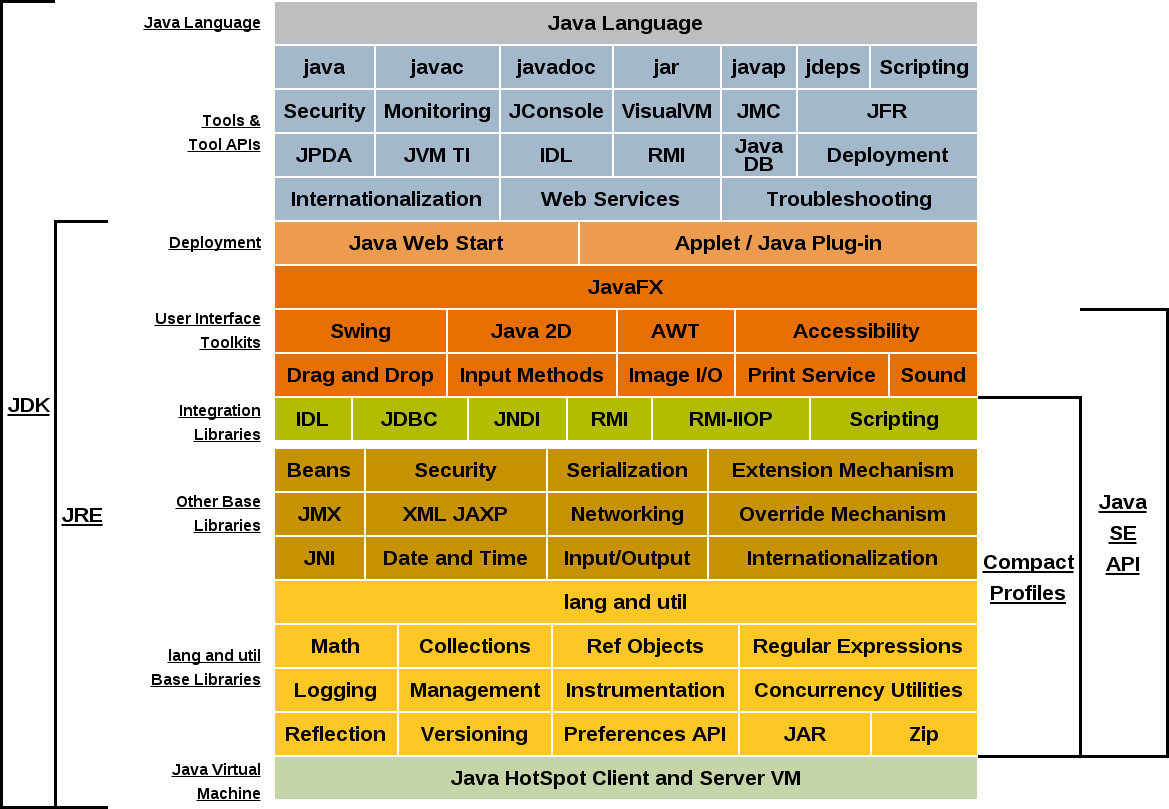
\includegraphics[scale=0.3]{fig/java_jdk.jpg}
    \caption{Java SE JDK 1.8}
\end{figure}



\section{Android}
Android je mobilní operační systém vyvíjený společností Google, který je založený na Linuxovém jádře. Je vyvíjen jako opensource a používá se především v mobilních zařízeních jako jsou chytré telefony, hodinky a tablety. Můžeme jej však také nalézt také v přístrojích jako jsou set-top boxy, multimediální přehrávače a v jiné elektronice.\\
\subsection{Historie}
Počátky Androidu spadají do roku 2003, kdy byla v Kalifornii v USA založena společnost Android, Inc. O Dva roky později firmu odkupuje světoznámá společnost Google. V roce 2007 získává Google několik patentů v oblasti mobilních zařízení a 5. listopadu téhož roku dochází k oficiálnímu představení a vzniká sdružení firem Open Handset Alliance, která mé za cíl vytvoření otevřených standartů v oblasti mobilních zařízení. V tabulce TODO odkaz je zobrazena stručná historie verzí operačního systému Android.

\begin {table}[h!]
\begin{tabular}{|l|c|l|c|}
\hline
{\bf Datum}         & {\bf Verze}   & {\bf Označení}        & {\bf Verze API}   \\
\hline \hline
23. září 2008       & 1.0 -- 1.1    & --                    & 1 -- 2            \\
\hline
April 27, 2009      & 1.5           & Cupcake               & 3                 \\
\hline
September 15, 2009  & 1.6           & Donut                 & 4                 \\
\hline
October 26, 2009    & 2.0 -- 2.1    & Eclair                & 5 -- 7            \\
\hline
May 20, 2010        & 2.2 -- 2.2.3  & Froyo                 & 8                 \\
\hline
December 6, 2010    & 2.3 -- 2.3.7  & Gingerbread           & 9 -- 10           \\
\hline
February 22, 2011   & 3.0 -- 3.2    & Honeycomb             & 11 -- 13          \\
\hline
October 18, 2011    & 4.0 -- 4.0.4  & Ice Cream Sandwich    & 14 -- 15          \\
\hline
July 9, 2012        & 4.1 -- 4.3    & Jelly Bean            & 16 -- 18          \\
\hline
October 31, 2013    & 4.4           & KitKat                & 19 -- 20          \\
\hline
November 12, 2014   & 5.0           & Lollipop              & 21                \\
\hline
\end{tabular}
\centering
\caption{Verze operačního systému Android}
\end{table}

\subsection{Arcitektura}
Architektura systému android je složena z šesti vrstev:
\begin{itemize}
\item Linuxové jádro
\item HAL
\item Knihovny
\item Android runtime
\item Application framework
\item Aplikace
\end{itemize}
\subsubsection{Linuxové jádro} %https://source.android.com/devices/
Tato nejnižší vrstva je postavena mezi hardware zařízení a ostatní vrstvy architektury. Android je postavený na zvlaštní verzi Linuxového jádra a několika speciálními doplňky jako jsou správa systémové paměti, the Binder IPC driver, and other. Od počátku byl android postaven na linuxovém jádru 2.6, nejnověší android pak běží na jádru 3.4.  Při startu se jádro zavede do operační paměti a je mu předáno řízení.
\subsubsection{Hardware abstraction layer (HAL)} %https://source.android.com/devices/
HAL je standartní rozhraní které umožňuje systému android volat do vrstvy ovladačů, zatímco je mu jedno jaká je implementace v nižších vrstvách obladačů a hardwareru. Pro každý kus hardwaru by měl existovat ovladač a k němu odpovídající HAL poskytující možnosti hardwaru.
\subsubsection{Knihovny}
Nad HAL vrstvu se nachází vrstva nativních knihoven. Tyto knihovny jsou napsány v jazyce C nebo C++. K těmto knihonám se dá přistoupit přes android sdk pokud je však požadován přímý přístup je možné to provést přes NDK. Mezi tyto knihovny patří:
\begin{itemize} %http://www.android-app-market.com/android-architecture.html
\item Surface manager -- knihovna pro skládání oken na obrazovce
\item Media Framework -- poskytuje různé multimediální kodeky pro nahrávání a přehrávání videa v různých formátech.
\item SQLite -- databázový engine pro použítí v oblasti uložení dat
\item WebKit -- prohlížečový enginepro  zobrazování webového obsahu
\item Libc -- standartní knihovna jazyka C 
\item OpenGL ES -- knihovna pro podporu 2D a 3D grafiky a renderování.
\item Audio Manager -- knihovna pro práci se zvuky zařízení
\item FreeType -- knihovna pro bitmapové a vektorové vykreslení písma
\item SSL -- knihovna pro využití šifrovacího protokolu pro bezpečnou intenetovou komunikaci.
\item and others.
\end{itemize}


\subsubsection{Android runtime}
Vedle vrstvy nativních knihoven se nachází se nachází Android Runtime vrstva, která se skládá ze dvou základních částí a to z Core Libraies a z Dalvik Virtual Machine (DVM). \\
Core libraries jinak řečené Android API se skládají z tří hlavních částí



\subsubsection{Application framework}
Vrstva aplikačního frameworku poskytuje mnoho vysoko-úrovňových služeb aplikacím ve formě java knihoven. Pro vývojáře se jedná o nejdůležitější vrstvu,která umožňuje přístup ke službám daného zařízení. Tato vrstva je tvořena: 
\begin{itemize} %http://developer.android.com/reference/
\item Activity manager -- ovládání životního cyklu aplikací jejich start průběh a konec
\item Windows manager -- pro správu viditelnosti oken a jejich uspořádání
\item Content Providers -- umožňuje pracovat s obsahem jiných aplikací, poskytuje mechanismy pro jejich zabezpečení 
\item View System -- View je základní stavební blok pro komponenty uživatelského rozhraní. View systém je sada View která slouží k budování uživatelského rozhraní aplikace.
\item Notification manager -- Umožňuje uživatele informovat pomocí alertů a notifikací.
\item Package manager -- Umožňuje získat různé informace o aplikacích které jsou aktuálně naisntalovány  zařízení.
\item Telephony manager -- Poskytuje přístup k telefoním službám zařízení. 
\item Resource manager -- Umožňuje přístup ke zdrojům jako jsou barevná nastavení, rozvržení a stringy.
\item Location manager - Poskytuje přístup k systémovým lokačním službám. Tyto služby umožňují v pravidelných intervalech získávat geografick souřadnice zařízení.
\item and others.
\end{itemize}

\subsubsection{Aplikace}
Poslední a nejvyšší vrstva se skládá ze samotných aplíkací. Jendak se jedná o předinstalované aplikace a druhak se jedná o aplikace, které byly postupem času přidány z android obchodu nebo jinou cestou.

\begin{figure}[h!]
    \centering
    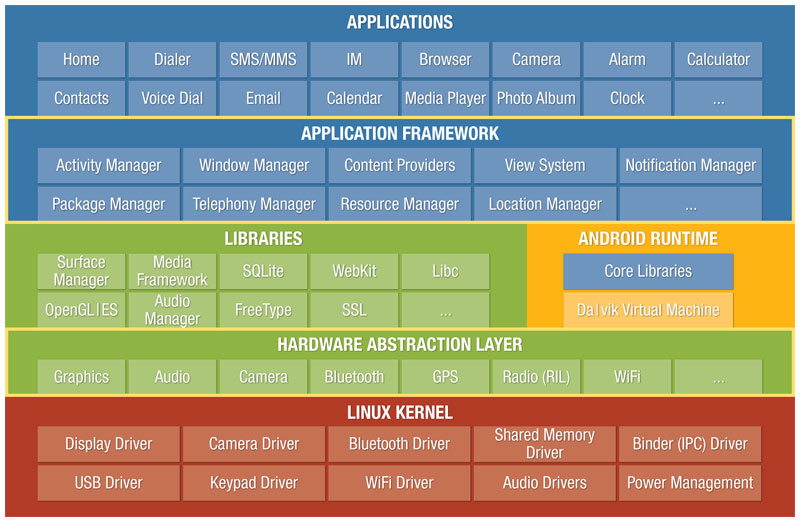
\includegraphics[scale=0.5]{fig/android_architecture.jpg}
    \caption{Android architecture}
\end{figure}

\section{Gradle}


\section{JBoss Drools}

  \subsection{Drools Expert}

  \subsection{OptaPlanner}


\section{Vehicle routing problem}

%\subsection{History}
%V následující tabulce je stručně popsána historie programovacího jazyku Java: \\
%\\
%\begin {table}[h!]
%\begin{tabular}{|l|l|l|}[h]
%\hline
%    {\bf Název} & {\bf Datum} & {\bf Poznámka}  \\
%    \hline \hline
%    Oak         & 1991                  & a     \\
%    JDK         & 1995                  & a     \\
%    JDK 1.0     & January 23rd, 1996    & a     \\
%    JDK 1.1     & February 19th, 1997   & a     \\
%    JPE         & May, 1998             & a \\
%    J2SE 1.2    & December 8th, 1998    & a     \\
%    J2EE 1.2    & December 12, 1999     & a     \\
%    J2SE 1.3    & May 8th, 2000         & a     \\
%    J2EE 1.3    & September 24, 2001    & a \\
%    J2SE 1.4    & February 6th, 2002    & a     \\
%    J2EE 1.4    & November 11, 2003     & a \\
%    J2SE 5.0    & September 30th, 2004  & a     \\
%    Java EE 5   & May 11, 2006          & a \\
%    Java SE 6   & December 11th, 2006   & a     \\
%    Java EE 6   & December 10, 2009     & a \\
%    Java SE 7   & July 28th, 2011       & a     \\
%    Java EE 7   & June 12, 2013         & a \\
%    Java SE 8   & March 18th, 2014      & a     \\
%  \hline
%\end{tabular}
%\caption{Historie Javy}
%\end{table}




